\section{Runtime Inefficiencies}
\label{removal}

When submitting a job or application for execution on a given computing system, most users trust the default configurations of the submission environment. However, if the user needs to improve the efficiency of the code execution, he/she must be aware of the environment variables that can be controlled and how those can impair the performance. Two cases will be addressed here: (i) how to spread the code parallelism, between processes and threads, and (ii) how to allocate the available cores on each device to threads and processes.

\subsection{Multithreading Inefficiencies}

Without the sensibility provided by the tests in section \ref{identification}, a scientist would incur in the pitfall of using all available cores on the system (and even all hardware threads, if each core supports hardware multithreading), hoping that it would provide the best performance. While it may be true for the non-pointer implementation, the system computational resources would be inefficiently used, and using the single device highly efficient pointer implementation would induce a even greater waste.

A closer look to the pointer based implementation shows in fact that it is the most efficient one. As seen in section \ref{data_inef}, the scalability of the parallelization is limited by the NUMA organization on modern multiple CPU device systems. If the threads on $cpu_1$ do not share information with the threads on $cpu_2$, the NUMA bottleneck is removed by using multithreaded processes. However, parallelization at the process level, where each process performs a data analysis on a separate event, is not possible with the current implementation of LipMiniAnalysis, where a single global state is allocated to store data from each event processing.

\begin{figure}[!htp]
	\begin{center}
		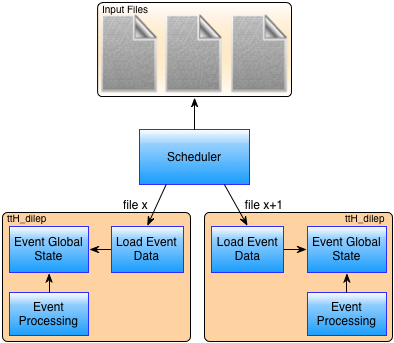
\includegraphics[scale=0.5]{images/scheduler_workflow.png}
		\caption{Schematic representation of dispatcher workflow.}
		\label{fig:sched_flow}
	\end{center}
\end{figure}

Data analysis applications are individually executed for each file (around 1GB in size) in a very large set of files, at a terabyte scale, received weekly from CERN. An alternative approach to the process parallelization over a single input data file is to balance the execution of different \tth processes in the system on a set of distinct input files. This reduces the complexity of the implementation, with no changes needed for \tth, and avoids communication between processes. A simple scheduler was devised, which takes a set of input files and spawns a given amount of \tth processes. The scheduler dispatches the files to the different processes in a queue-like approach, and monitor their execution as shown in figure \ref{fig:sched_flow}. A set of 20 input files was considered for testing and evaluation purposes, with different configurations of processes and threads per process.

Figure \ref{fig:Sched} presents the speedups using 2, 4, 5, 8, and 10 processes for various thread configurations, with maximum number of threads limited to 40. A higher amount of processes was not tested as the efficiency decayed from 8 to 10 processes. The best speedups occur for 8 processes with 5 threads each, with a peak of 69.3, 7.8 and 11.7 times better than the best non-pointer and pointer implementations, respectively. A small number of threads such as this allows for a small overhead in the \tth parallelization, namely on load balancing and final best reconstruction merge for each event. For 10 processes the load on the system due to the lack of shared memory and I/O operations affects the performance, decreasing the speedups relatively to using 8 processes. A common behaviour is that when using the CPU devices hardware multithreading the speedups tend to stabilize, or even drop for 2, 4, and 5 processes. Overall, the best speedups occur when using all available cores on the system, with multithreading.

\begin{figure}[!htp]
	\begin{center}
		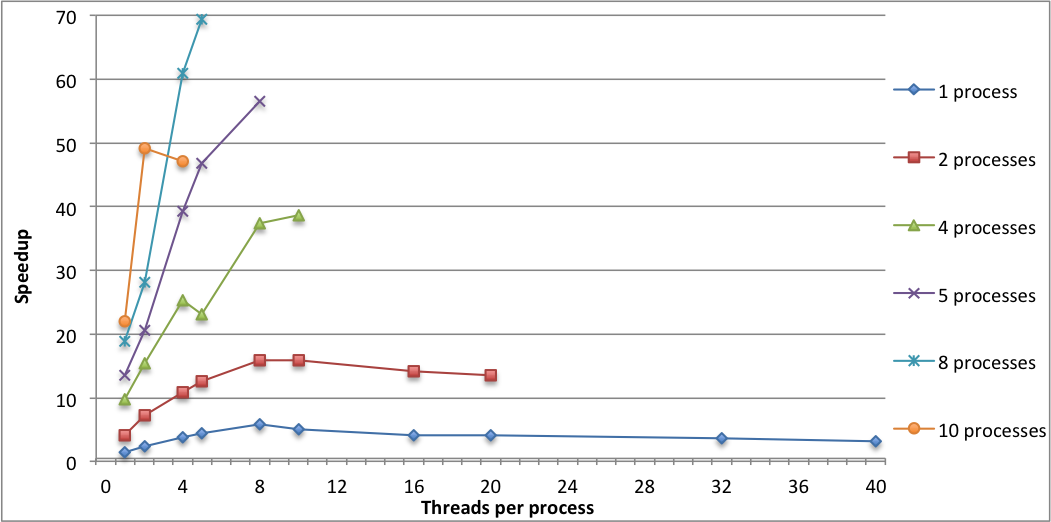
\includegraphics[scale=0.5]{charts/speedup_sched.png}
		\caption{Speedups for the scheduler with the pointer based implementation for several combinations of \#processes and \#threads per process.}
		\label{fig:Sched}
	\end{center}
\end{figure}

\subsection{Core Affinity Inefficiencies}

One of the key issues in runtime efficiency is the thread affinity \cite{Affinity}, namely to control the allocation of each thread to which CPU core. By default, OpenMP lets the operating system to manage the thread affinity; as a consequence, threads may migrate among cores during runtime. If a thread is running on core $c_1$ and moves to core $c_2$, all data on the private cache $l_{c_1}$ needs to be reloaded to cache $l_{c_2}$, causing unnecessary overhead. This effect is amplified if the threads are moved between adjacent CPU devices. When multiple different, and (possibly) parallel processes are running on the same system, which is common in production environments, such scheduling occurrences happen more frequently. This subsection presents a preliminary study on thread affinity for data analysis code.

Defining the thread affinity of an application may provide a more predictable, or in some cases better, performance. In theory, an optimum thread affinity scheme allocates the threads to contiguous physical cores of one CPU device, uses the cores of the second CPU device only after the first is filled, and finally uses the multithreading capability after filling all physical cores. Note that using multithreading before the second CPU device is fully occupied may provide better performance in memory bound applications. This type of affinity must be defined prior to the application execution and depends on the system used. In this compute bound data analysis case, the affinity was specifically tuned to the 20-core testbed system for all threads or process/threads configurations for the scheduler.

\begin{figure}[!htp]
	\begin{center}
		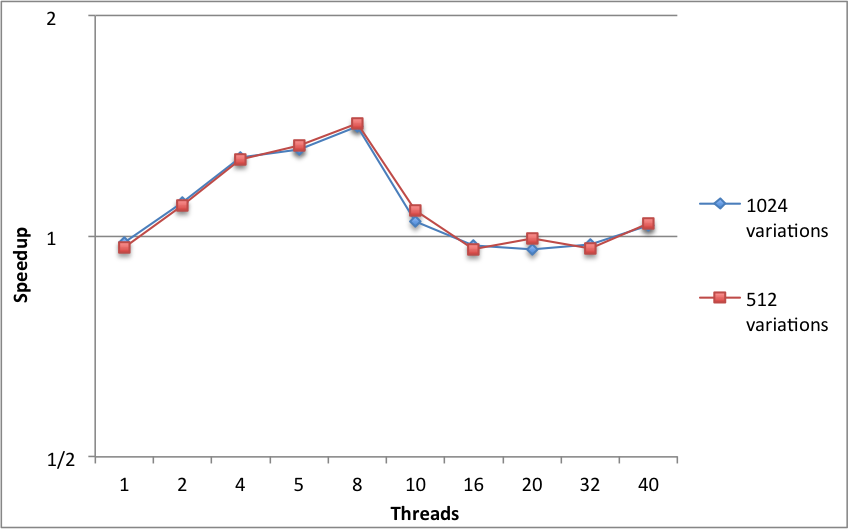
\includegraphics[scale=0.55]{charts/speedup_pointer_aff.png}
		\caption{Speedup of the \tth parallel pointer implementation with core affinity.}
		\label{fig:pointer_aff}
	\end{center}
\end{figure}

By analysing the speedups of the pointer implementation of \tth with thread affinity, in figure \ref{fig:pointer_aff}, the specification of the affinity provides speedups for the previous most efficient number of threads, i.e., up to 8 threads. For 8 threads the performance increases by 41\%, relative to its no affinity counterpart. With this number of threads, and the amount of shared data, moving threads between cores at runtime causes more cache warm ups to occur, significantly affecting the performance. When using more than 10 threads the application is roughly 4\% slower as the operating system uses some multithreaded cores rather than using all available physical cores and it does a better job at managing the multithreading.

The same affinity study was performed on the scheduler, with the speedups presented in figure \ref{fig:sched_aff}. The performance is increased for some specific configurations, with the exception of 5 processes that is always worse, providing improvements up to 52\%, 90\%, 8\%, and 25\% for 2, 4, 8, and 10 processes respectively.

\begin{figure}[!htp]
	\begin{center}
		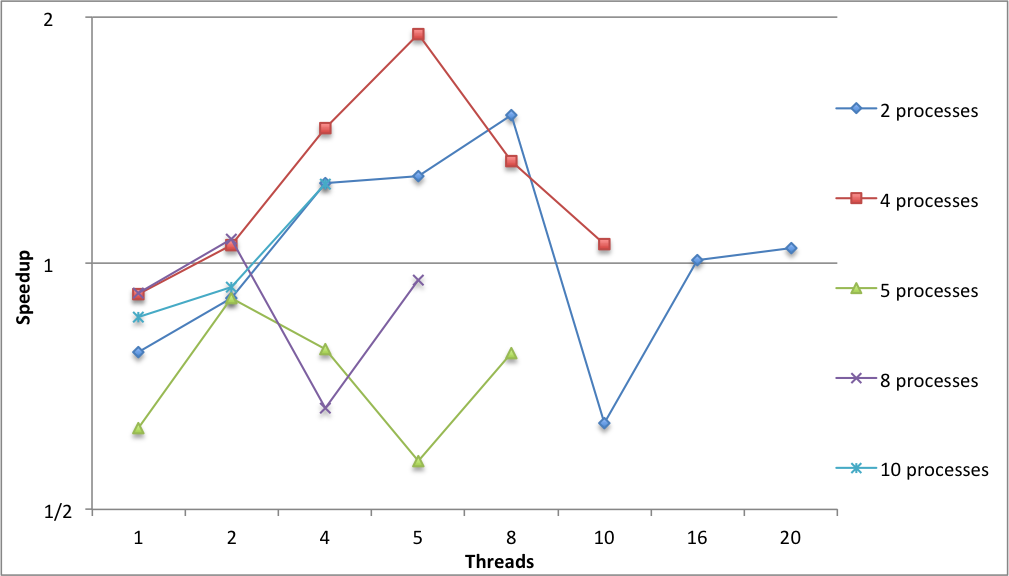
\includegraphics[scale=0.55]{charts/speedup_sched_aff_1024.png}
		\caption{Speedups of the scheduler with the pointer based implementation for various threads per process with core affinity.}
		\label{fig:sched_aff}
	\end{center}
\end{figure}

The performance with core affinity is less susceptible to oscillations, as with no affinity it is sometimes affected by OS thread reallocations. It is when many reallocations may occur that setting the core affinity provides the best performance. Hard setting the affinity may not allow for proper multithreading to hide the memory accesses latency, affecting the performance. It is not possible to use a theoretical affinity scheme to always improve the performance on every system, as it is highly dependent on:

\begin{itemize}
	\item the algorithm, memory bound, suffers more from core reallocation due to losing all data on cache, where fixing their position on a specific core avoids unnecessary accesses to the RAM;
	\item the application execution time, as the impact from thread reallocations is higher in applications with low execution times;
	\item the operating system, as OpenMP, by default, lets it manage the thread allocation and it is susceptible to the overall system load, causing fluctuations in consecutive applications execution time.
\end{itemize}

With all optimizations considered, the best overall performance in a dual 10-core Xeon system is obtained using the scheduler combined with the pointer implementation, with 8 multithreaded processes (with 5 threads each), reaching a speedup of 113 over the original sequential application.
